\documentclass[ucs, notheorems, handout]{beamer}

\usetheme[numbers,totalnumbers,nologo]{Statmod}
\usefonttheme[onlymath]{serif}
\setbeamertemplate{navigation symbols}{}

\mode<handout> {
    \usepackage{pgfpages}
    \setbeameroption{show notes}
    % \pgfpagesuselayout{2 on 1}[a4paper, border shrink=5mm]
    \setbeamercolor{note page}{bg=white}
    \setbeamercolor{note title}{bg=gray!10}
    \setbeamercolor{note date}{fg=gray!10}
}

\usepackage[utf8x]{inputenc}
\usepackage[T2A]{fontenc}
\usepackage[russian]{babel}
% \usepackage{tikz}
% \usepackage{ragged2e}
% \usepackage{wrapfig}
% \usepackage{graphicx}

% \graphicspath{ {images/} }
\usepackage{graphicx}
\graphicspath{ {images/} }

\usepackage{amsmath}
\usepackage{amsfonts}
\usepackage{bm}

% \usepackage{fig}
\usepackage{subcaption}


% \title[Решение задачи принятия решений]{Разработка программных средств и решение задач принятия решений с помощью методов тропической математики}

% \author{Кривулин Н.К., Ткаченко Е.А. СПбГУ}

% \institute[Санкт-Петербургский Государственный Университет]{%
%     \small
%     д.ф.-м.н., профессор Кривулин Николай Кимович\\ Ткаченко Егор Андреевич \\ \vspace{0.5cm}
%     Санкт-Петербургский государственный университет\\
%     Кафедра статистического моделирования}


\makeatletter
\defbeamertemplate*{footline}{infolineslong}
{
  \leavevmode%
  \hbox{%
  \begin{beamercolorbox}[wd=.3\paperwidth,ht=2.5ex,dp=1ex,center]{author in head/foot}%
    \usebeamerfont{author in head/foot}\insertshortauthor\expandafter\beamer@ifempty\expandafter{\beamer@shortinstitute}{}{~~(\insertshortinstitute)}
  \end{beamercolorbox}%
  \begin{beamercolorbox}[wd=.55\paperwidth,ht=2.5ex,dp=1ex,center]{title in head/foot}%
    \usebeamerfont{title in head/foot}\insertshorttitle[width=\textwidth, respectlinebreaks]
  \end{beamercolorbox}%
  \begin{beamercolorbox}[wd=.15\paperwidth,ht=2.5ex,dp=1ex,right]{date in head/foot}%
%    \usebeamerfont{date in head/foot}\insertshortdate{}\hspace*{2em}
\insertframenumber{} / \inserttotalframenumber\hspace*{2ex} 
  \end{beamercolorbox}}%
  \vskip0pt%
}

\uselanguage{Russian}
\languagepath{Russian}


\makeatother
\title[Разработка ПО и решение задач принятия решений]{Разработка программных средств и решение задач принятия решений с помощью методов тропической математики}
\author{Ткаченко Егор Андреевич}
\institute[]{
    \small{Санкт-Петербургский государственный университет \\
Прикладная математика и информатика \\
Вычислительная стохастика и статистические модели \\
\vspace{0.5cm}
\textbf{Научный руководитель:}  д.ф.-м.н., профессор Н.\,К.~Кривулин \\
\textbf{Рецензент:} Старший преподаватель, Высшая школа
интеллектуальных систем и
суперкомпьютерных технологий СПбПУ
Петра Великого В. А. Пархоменко}
}


    % \title[Решение задачи принятия решений]{Разработка программных средств и решение задач принятия решений с помощью методов тропической математики}

    % \author{Ткаченко Егор Андреевич, гр.19.Б04-мм}
    
    % \institute[Санкт-Петербургский Государственный Университет]{%
    %     \small
    %     Санкт-Петербургский государственный университет\\
    %     Прикладная математика и информатика\\
    %     Вычислительная стохастика и статистические модели\\
    %     \vspace{1.25cm}
    %     Отчет по преддипломной практике (семестр 8)}
    
    % \date[Зачет]{Санкт-Петербург, 2023}


% \title[Решение задачи принятия решений]{Разработка программных средств и решение задач принятия решений с помощью методов тропической математики}
% \author{Ткаченко Егор Андреевич, гр. 422}
% \institute{Санкт-Петербургский государственный университет \\
%     Математико-механический факультет \\
%     Кафедра статистического моделирования \\
%     \vspace{0.7cm}
%     Научный руководитель:  д.ф.-м.н. Кривулин Н.К.  \\
%     Рецензент: ??????? \\
%     \vspace{0.7cm}
% }
% \date{
%     Санкт-Петербург\\
%     2023г.
% }



\begin{document}

% \setbeameroption{show notes}
\setbeameroption{hide notes}

\begin{frame}
    % \begin{frame}[plain]
    \titlepage

    \note{Научный руководитель  д.ф.-м.н., доцент Кривулин Николай Кимович,\\
    кафедра статистического моделирования}
\end{frame}




\begin{frame}{Введение}
    \begin{itemize}
        \item Рассматриваются задачи в которых на основе парных сравнений альтернатив требуется найти их абсолютный приоритет.

        \item Для решения существует два подхода --- эвристические алгоритмы и аналитические методы.
    
        \item Одним из аналитических решений является метод аппроксимации матрицы парных сравнений в log-чебышевской метрике. 

        \item Указанный метод позволяет найти аналитическое решение в терминах max-алгебры.
    
        \item Цели работы --- решение задач принятия решений и разработка алгоритмов, способа хранения данных и программных средств, предназначенных для решения задачи принятия решений.
    \end{itemize}
    
    \note{В работе рассматриваются задачи принятия решений на основе парных сравнений.

    Методы решения этих задач можно отнести к двум подходам - эвристические методы (эвристические значит не гарантирующие точного решения, но зачастую работающие быстрее) и аналитические.
    
    Одно из таких аналитических решений - метод аппроксимации в log-чебышевской метрике.
    
    этот  метод очень позволяет найти аналитическое решение в терминах max-алгебры.
    
    Цель работы - разработка алгоритмов, способа хранения данных и программных средств, предназначенных для решения задачи принятия решений}
\end{frame}


\begin{frame}
    \frametitle{Задачи принятия решений}


    \begin{block}{Многокритериальная задача}
        \begin{itemize}
            \item Имеются $n$ альтернатив $\mathcal{A}_{1},\ldots,\mathcal{A}_{n}$ принятия решения.
            \item Имеются $m$ критериев и для каждого дана матрица $\bm{A}_{k} = (a_{ij}^{(k)})$ парных сравнений альтернатив.
            \item $a_{ij}^{(k)}>0$ показывает во сколько раз альтернатива $\mathcal{A}_{i}$ превосходит альтернативу $\mathcal{A}_{j}$ в соответствии с критерием $k=1,\ldots,m$.
            \item Дана матрица попарных сравнений критериев $\bm{C}=(c_{kl})$, где $c_{kl}$ показывает во сколько раз критерий $k$ важнее $l$.
            \item Требуется на основе матриц $\bm{C}$ и $\bm{A}_{1},\ldots,\bm{A}_{m}$ определить вектор $\bm{x}$ абсолютных рейтингов альтернатив.
        \end{itemize}
    \end{block}

    \note{Подробнее про задачу:

    имеются альтернативы принятия решений, например какого типа построить мост (арочный, балочный, висячий).
    
    Имеются критерии например (цена, сложность время строительства)
    
    для каждого критерия дана матрица парных сравнений альтернатив, которая может быть получена например опросом экспертов, а  парных потому что экспертное мнение будет точнее при выборе из 2 альтернатив чем из нескольких
    
    элементы этих матриц отображают во сколько одна альтернатива лучше другой по каждому критерию.
    
    Так же дана матрица парных сравнений критериев, элементы которой показывают во сколько один критерий важнее другого.
    
    Задача - построить вектор абсолютных рейтингов альтернатив.}
\end{frame}

% \begin{frame}
%     \frametitle{Элементы тропической математики}

% \end{frame}

\begin{frame}
    \frametitle{Элементы тропической математики}
    \begin{block}{Max-алгебра}
        Множество $\mathbb{R}_+ = \{x \in \mathbb{R} \, |\, x \geq 0\}$ с операциями сложения и умножения.
    \end{block}
    \begin{itemize}
        \item Сложение обозначается символом $\oplus$ и для всех $x,y\in\mathbb{R}_{+}$ определено как максимум: $x\oplus y=\max\{x,y\}$.
        \item Сложение обладает свойством идемпотентности: $x\oplus x=x$.
        \item Умножение определено и обозначается как обычно.
        \item Нейтральные элементы по сложению и умножению совпадают с арифметическими нулем и единицей.
        \item Понятия обратного элемента по умножению и степени числа имеют обычный смысл. 
    \end{itemize}

    \note{Про максалгебру:

    Макс-умножить алгебра - это множество неотрицательных чисел с операциями сложения и умножения.
    
    Сложение обозначается символом оплюс, и определено как максимум.
    
    так же сложение идемпотентно.
    
    Умножение определено и обозначается как обычно для вещественных чисел.
    
    нейтральные элементы - 0 для сложения (как наименьший из множества) и 1 для умножения (как в классической алгебре)
    
    Возведение в степень определено как обычно, в том числе обратный элемент как -1 степень.}
\end{frame}

\begin{frame}
    \frametitle{Матрицы в max-алгебре}
    \begin{itemize}
        \item Векторные и матричные операции, в том числе операции умножения на скаляр и возведение в натуральную степень, выполняются по стандартным правилам с заменой арифметического сложения на операцию $\oplus$. 
        % Нулевой вектор, который обозначается символом $\bm{0}$, нулевая матрица, а также положительный вектор имеют стандартный вид.
        
        % \item Для ненулевого вектора-столбца $\bm{x}=(x_{j})$ определен мультипликативно сопряженный вектор-строка $\bm{x}^{-}=(x_{j}^{-})$, где $x_{j}^{-}=x_{j}^{-1}$, если $x_{j}\ne0$, и $x_{j}^{-}=0$ в противном случае.
        
        
        
        \item След матрицы $\bm{A}=(a_{ij})$ порядка $n$ вычисляется по формуле
        $$\mathop\mathrm{tr}\bm{A}=a_{11}\oplus\cdots\oplus a_{nn}.$$

        \item Спектральный радиус матрицы $\bm{A}$ определяется выражением
        \begin{equation*}
        \lambda
        =
        \mathop\mathrm{tr}\bm{A}\oplus\cdots\oplus\mathop\mathrm{tr}\nolimits^{1/n}(\bm{A}^{n})
        =
        \bigoplus_{i=1}^{n}{\mathop\mathrm{tr}}^{1/i}(\bm{A}^{i}).
        \end{equation*}

        \item При $\lambda\leq1$, определен оператор Клини матрицы $\bm{A}$ в виде
        \begin{equation*}
        \bm{A}^{\ast}
        =
        \bm{I}\oplus\bm{A}\oplus\cdots\oplus\bm{A}^{n-1}
        =
        \bigoplus_{i=0}^{n-1}\bm{A}^{i}.
        \end{equation*}
    \end{itemize}

    \note{операции с матрицами и векторами определятся как обычно, с заменой арифметического сложения на операцию оплюс.

    Вводятся такие понятия как:
    
    След - максимальный элемент на диагонали.
    
    Спектральный радиус - максимальное собственное число, в терминах максалгебры записывается как вот такая сумма.
    
    Когда спектральный радиус матрицы меньше или равен 1, для нее можно определить оператор клини. он обозначается звездочкой.}
\end{frame}

\begin{frame}
    \frametitle{\large{Решение задачи парных сравнений (Krivulin N. et al. 2022)}}
    \begin{itemize}
        \item[1] На основе матрицы $\bm{C}$ находится вектор весов критериев $\bm{w}$
        $$\bm{w} =
        (\lambda^{-1}\bm{C})^{\ast}\bm{v},
        \qquad \bm{v}>\bm{0},
        \qquad \lambda =
        \bigoplus_{i=1}^{m}{\mathop\mathrm{tr}}^{1/i}(\bm{C}^{i}).$$
        \item[2] Если вектор $\bm{w}$ не единственный (с точностью до положительного множителя), то определяются наилучший $\bm{w}_{1}$ и наихудший $\bm{w}_{2}$ дифференцирующие векторы весов.
        \item[3]
        С помощью векторов $\bm{w}_{1}=(w_{i}^{(1)})$ и $\bm{w}_{2}=(w_{i}^{(2)})$ строятся взвешенные суммы матриц парных сравнений альтернатив:
        $$\bm{B} =
        \bigoplus_{i=1}^{m}w^{(1)}_{i}\bm{A}_{i},
        \qquad \bm{D} =
        \bigoplus_{i=1}^{m}w^{(2)}_{i}\bm{A}_{i}.$$
        \item[4.]
        Повторяя действия пунктов 1 и 2 для матрицы $\bm{B}$, вычисляется наилучший вектор рейтингов альтернатив, а для матрицы $\bm{D}$ --- наихудший вектор.
 
    \end{itemize}

    \note{Определив базовые элементы максалгебры, можно рассмотреть алгоритм решения задачи парных сравнений.

    1) Сначала матрица парных сравнений критериев делится на свое собственное число и находится ее матрица клини.
    Линейная комбинация столбцов полученной матрицы является вектором весов критериев.
    
    2) Если такой вектор не единственный с точностью до умножения на скаляр, то выбирается наилучший и наихудший дифференцирующий векторы.
    
    3) С выбранными весами критериев строятся взвешенные матрицы парных сравнений альтернатив и для них повторяются действия пунктов 1 и 2.
    
    4) Повторяя действия пунктов 1 и 2 для матрицы B,
    вычисляется наилучший вектор рейтингов альтернатив, а
    для матрицы D — наихудший вектор.
    
    В итоге получаются наилучший и наихудший дифференцирующий векторы рейтингов альтернатив.
    
    Наилучших и наихудших векторов может быть несколько.}
\end{frame}

\begin{frame}
    \frametitle{Разработка структуры для хранения чисел}

    \begin{itemize}
        \item Требуется структура основанная на целочисленных типах с точными операциями, например, для проверки на линейную независимость векторов.
        \item Введен класс объектов, характеризующийся тройками целых чисел.
    \end{itemize}
    \begin{block}{Структура}
        $$\displaystyle \left(\frac{a}{b}\right)^{1/n}, \quad a \in \mathbb{N} \cup 0, \quad b \in \mathbb{N}, \quad \gcd(a, b) = 1, \quad n \in \mathbb{N}$$
    \end{block}
    \begin{itemize}
        \item Введенный класс объектов с операциями сложения и умножения определяет алгебраическую систему, замкнутую относительно сложения, умножения, извлечения корня.
    \end{itemize}

    \note{проверки на линейную независимость векторов требуют структуру основанную на целочисленных типах, с точными операциями

    Поэтому был предложен класс объектов, характеризующийся тройками целых чисел.
    
    предложенный класс объектов с операциями сложения (максимума) и умножения определяет алгебраическую систему, замкнутую
    относительно сложения, умножения, извлечения корня.
    
    
    этой алгебраической системы достаточную для решения задачи парных сравнений при условии, что во входных матрицах --- рациональные числа в рациональной степени.}

\end{frame}

\begin{frame}
    \frametitle{Структуры для хранения чисел}
    \begin{block}{Структура A}
        $$\displaystyle \left(\frac{a}{b}\right)^{1/n}, \quad a \in \mathbb{N} \cup 0, \quad b \in \mathbb{N}, \quad \gcd(a, b) = 1, \quad n \in \mathbb{N}$$
    \end{block}
    $$\tilde{n}_1 = n_1 / \gcd(n_1, n_2), \qquad \tilde{n}_2 = n_2 / \gcd(n_1, n_2).$$
    % $$n_1 =  \tilde{n}_1 \cdot \gcd(n_1, n_2), \qquad n_2 =  \tilde{n}_2 \cdot \gcd(n_1, n_2).$$
    \begin{itemize}
        \item Умножение
        $$ \left(\frac{a_1}{b_1}\right)^{1/n_1} \times \left(\frac{a_2}{b_2}\right)^{1/n_2} = \left(\frac{a_1^{\tilde{n}_2}a_2^{\tilde{n}_1}}{b_1^{\tilde{n}_2}b_2^{\tilde{n}_1}}\right)^{1/\tilde{n}_1\cdot \gcd(n_1, n_2) \cdot \tilde{n}_2}.$$
        После умножения $a_1^{\tilde{n}_2}a_2^{\tilde{n}_1}$ и $b_1^{\tilde{n}_2}b_2^{\tilde{n}_1}$ сокращаются на их НОД.
        \item Сравнение
        $$ \left(\frac{a_1}{b_1}\right)^{1/n_1} < \left(\frac{a_2}{b_2}\right)^{1/n_2} \Leftrightarrow
        {a_1^{\tilde{n}_2}}{b_2^{\tilde{n}_1}} < {a_2^{\tilde{n}_1}}{b_1^{\tilde{n}_2}}.$$
    \end{itemize}

    \note{Структура А и отражает все такие числа.

    Умножение определятся вот такой формулой с использованием наибольшего общего делителя для оптимизации.
    
    Для вычисления максимума достаточно определить операции сравнения. Вот так ее можно свести к целочисленным операциям и сравнению целых чисел.
    
    Извлечение корня и нахождение обратного работает очевидным образом.}
\end{frame}


\begin{frame}
    \frametitle{Структуры для хранения чисел}
    \begin{block}{Структура B}
        $$p_1^{a_1}p_2^{a_2}\dots p_k^{a_k}, \quad p_i \text{ --- простые}, \quad a_i \in \mathbb{Q}.$$
    \end{block}
    Структура реализуется вектором пар натуральных и рациональных чисел с отдельным состоянием для 0.
    \begin{itemize}
        \item Умножение реализуется слиянием векторов множителей.
        % Например:
        $$ 2^3 3^{-2} \times 3^2 5^{-1} = 2^3 3^{-2+2} 5^{-1} =  2^3 5^{-1}.$$

        \item
        Пусть $l$ --- наименьший общий множитель знаменателей степеней $a_i$, тогда точное сравнение: 
        $$a < b \Leftrightarrow a/b = p_1^{a_1}p_2^{a_2}\dots p_k^{a_k} < 1 \Leftrightarrow 
        p_1^{l a_1}p_2^{l a_2}\dots p_k^{l a_k} < 1 \Leftrightarrow $$
        $$\Leftrightarrow
        \prod_{i \in \{i | a_i > 0\}} p_i^{l a_i} < \prod_{j \in \{j | a_j < 0\}} p_j^{-l a_j}.
        $$
        Если вещественное приближение $a/b$ достаточно отличается от единицы, то точное сравнение не производится.

    \end{itemize}

    \note{Структура А имеет недостаток — с увеличением размера матриц, операция умножения замедляется, т.к. числа не помещаются в стандартные типы.

    Структура B факторизует числа, но может хранить рациональные степени. Если добавить отдельное состояние для 0, то структура полностью содержит множество чисел необходимое для решения задачи принятия решений.
    
    Умножение реализуется слиянием векторов множителей
    
    Для сравнения находится отношение чисел, далее вычисляется наименьший общий множитель знаменателей степеней, и все степени умножаются на него, чтобы быть целыми. Сравнение с единицей от этого не изменится.
    Остается только вычислить произведение простых с положительными и с отрицательными степенями отдельно и сравнить их.
    Но это медленная процедура и перед ней быстро вычисляется приближение отношения и если оно достаточно далеко от 1, то медленная процедура не запускается.}
\end{frame}

\begin{frame}
    \frametitle{Сравнение структур}
    \begin{itemize}
        \item Тест --- вычисление $(\lambda^{-1}\bm{A})^*$, где $\lambda$ --- спектральный радиус матрицы $\bm{A}$, $\bm{A}$ --- случайно сгенерированная матрица парных сравнений $n\times n$.
        \item Асимптотика такого теста --- $O(n^4 (t_\times + t_\oplus))$, где $t_\times, t_\oplus$ --- сложность (время) умножения и сложения чисел, соответственно.
        \item Для каждого значения $n$ проведено по 10 тестов и найдено среднее время вычисления в миллисекундах.
    \end{itemize}

    \note{Ожидается что Структура B медленнее с маленькими числами и быстрее с большими.

    Для проверки этого Сравню структуры во времени вычисления $(\lambda^{-1}\bm{A})^*$. Для случайно сгенерированных матриц парных сравнений A.
    
    Асимптотически там $O(n^4)$ операций сложения и умножения.
    
    Для каждого n от 10 до 100 с шагом 5 для каждой структуры проведено по 10 тестов. и получено время их выполнения в миллисекундах. все тестирование заняло 6 часов многопоточных вычислений.}
\end{frame}

\begin{frame}
    \frametitle{Результат сравнения}


%     \begin{figure}
%         \centering
%         \begin{subfigure}[b]{0.45\textwidth}
%             \centering
%             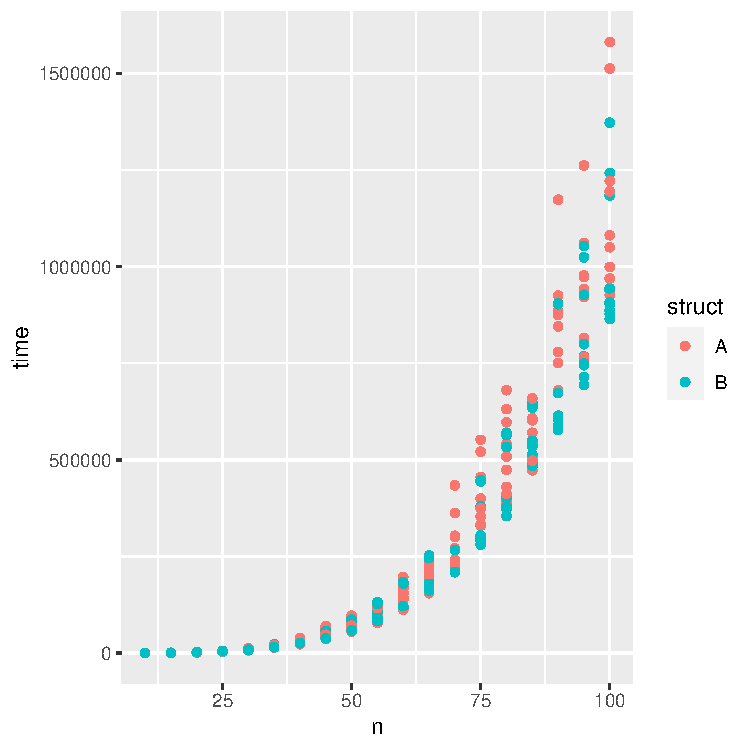
\includegraphics[width=\textwidth]{point.pdf}
%             \caption{$y=x$}
%             \label{fig:y equals x}
%         \end{subfigure}
%         \hfill
%         \begin{subfigure}[b]{0.45\textwidth}
%             \centering
%             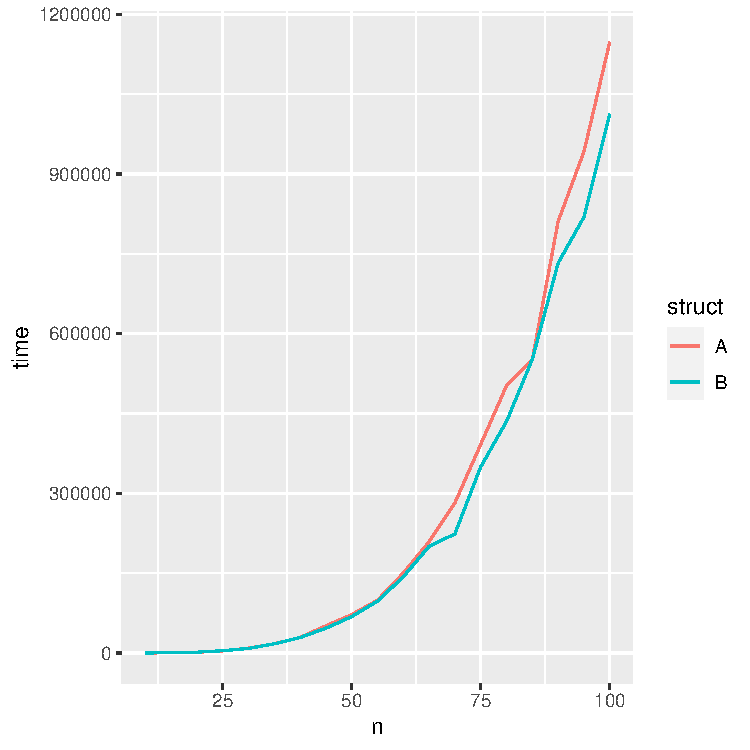
\includegraphics[width=\textwidth]{line.pdf}
%             \caption{$y=5/x$}
%             \label{fig:five over x}
%         \end{subfigure}
%            \caption{Three simple graphs}
%            \label{fig:three graphs}
%    \end{figure}

    \begin{figure}[h]
        \begin{subfigure}[t]{0.475\linewidth}%
            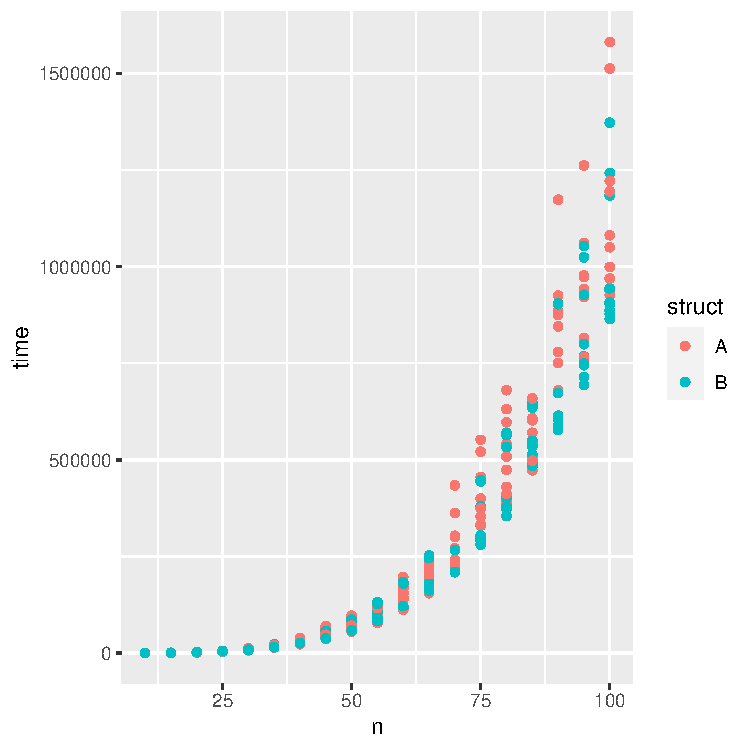
\includegraphics[width=\linewidth]{point.pdf}
            \caption{Все тесты}
        \end{subfigure}%
        \hfill
        \begin{subfigure}[t]{0.475\linewidth}%
            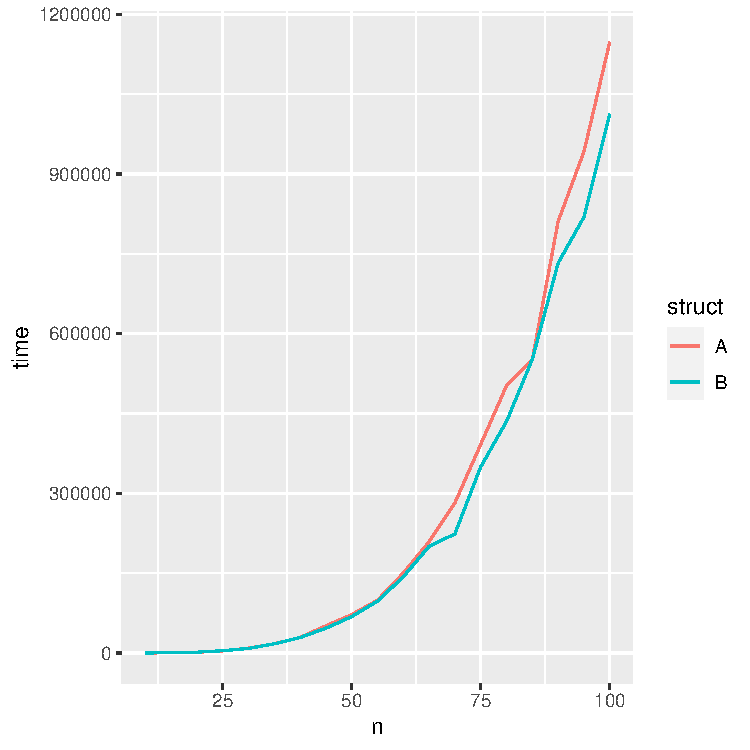
\includegraphics[width=\linewidth]{line.pdf}
            \caption{Среднее тестов}
        \end{subfigure}
    \end{figure}

    \note{По оси x - размер матриц n, по оси y - время вычисления теста.

    На левом графике изображены все тесты,
    
    На правом линии, проходящие через среднее время выполнения.

    Правый график хочется логарифмировать, но корректнее будет разделить на $n^4$ 
    }
\end{frame}

\begin{frame}
    \frametitle{Результат сравнения}
    \begin{figure}[h]
        \begin{subfigure}[t]{0.475\linewidth}%
            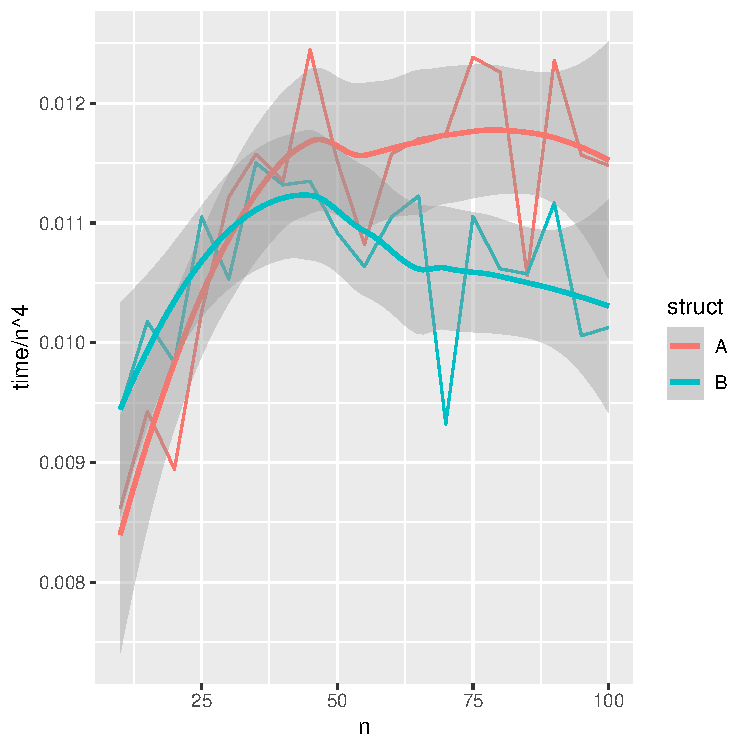
\includegraphics[width=\linewidth]{line_smooth_norm.pdf}
            \caption{Масштабирование по размеру матриц}
        \end{subfigure}%
        \hfill
        \begin{subfigure}[t]{0.475\linewidth}%
            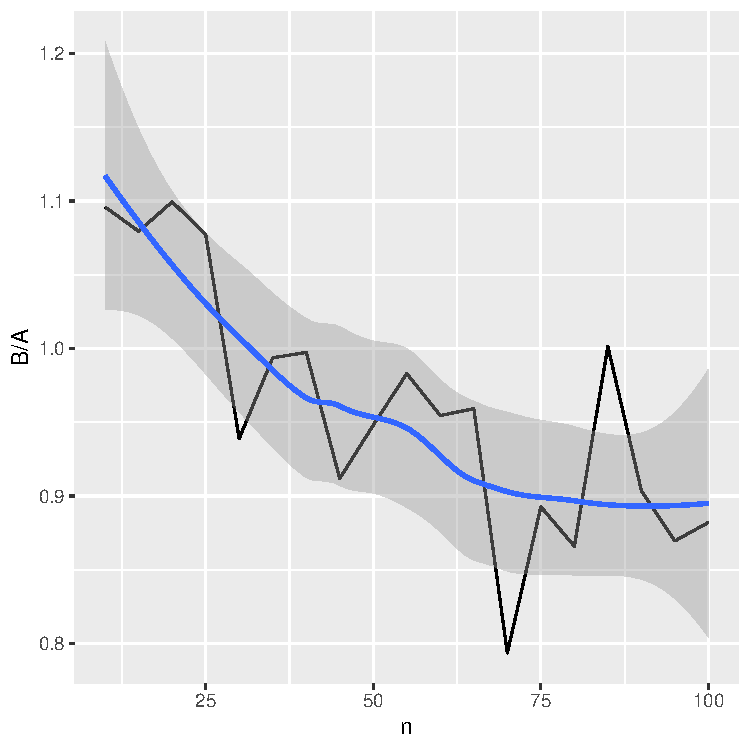
\includegraphics[width=\linewidth]{relation.pdf} 
            \caption{Отношение времени вычисления B и A}
        \end{subfigure}
    \end{figure}

    \begin{itemize}
        \item Структура A быстрее при маленьких $n$, начиная с $n = 30$, структура B быстрее.
        \item При размерах матрицы $n = 100$ структура B лучше на 10\%.
    \end{itemize}

    \note{получится левый график. По нему видно, что структура A быстрее при маленьких n, а начиная с n = 30,
    структура B быстрее.
    
    Если найти отношение времени выполнения B к A получится правый график, и из него видно, что при размерах матрицы n = 100 достигается преимущество структуры B на 10\%.}
\end{frame}

\begin{frame}
    \frametitle{Пример решения практической задачи}

$$\bm{C}= \begin{pmatrix}
1 & 3 & 7 & 5 & 1 & 7 & 1\\
1/3 & 1 & 9 & 1 & 1 & 5 & 1\\
1/7 & 1/9 & 1 & 1/7 & 1/5 & 1/2 & 1/4\\
1/5 & 1 & 7 & 1 & 1/4 & 7 & 1/3\\
1 & 1 & 5 & 4 & 1 & 5 & 3\\
1/7 & 1/5 & 2 & 1/7 & 1/5 & 1 & 1/6\\
1 & 1 & 4 & 3 & 1/3 & 6 & 1
\end{pmatrix}\!,
\bm{A}_1= \begin{pmatrix}
1 & 9 & 3\\
1/9 & 1 & 1/5\\
1/3 & 5 & 1
\end{pmatrix}\!,
$$
$$\bm{A}_2= \begin{pmatrix}
1 & 7 & 4\\
1/7 & 1 & 1/3\\
1/4 & 3 & 1
\end{pmatrix}\!,
\bm{A}_3= \begin{pmatrix}
1 & 1/5 & 1/3\\
5 & 1 & 2\\
3 & 1/2 & 1
\end{pmatrix}\!,
\bm{A}_4= \begin{pmatrix}
1 & 6 & 3\\
1/6 & 1 & 1/2\\
1/3 & 2 & 1
\end{pmatrix}\!,$$
$$
\bm{A}_5= \begin{pmatrix}
1 & 1/9 & 1/5\\
9 & 1 & 4\\
5 & 1/4 & 1
\end{pmatrix}\!,
\bm{A}_6= \begin{pmatrix}
1 & 1/7 & 1/4\\
7 & 1 & 3\\
4 & 1/3 & 1
\end{pmatrix}\!,
\bm{A}_7= \begin{pmatrix}
1 & 1/7 & 1/3\\
7 & 1 & 3\\
3 & 1/3 & 1
\end{pmatrix}\!.
$$

\end{frame}

\begin{frame}
    \frametitle{Результат работы программы}

$$\bm{x}_{best} =
\begin{pmatrix}
2^{2} 3^{-2}\\
2^{9/5} 3^{-19/10} 5^{1/5} 7^{-1/5}\\
1
\end{pmatrix} =$$
$$ = \begin{pmatrix}
(1048576/3486784401)^{1/10}\\
(6553600/56950811883)^{1/10}\\
1
\end{pmatrix} \approx
\begin{pmatrix}
0.44444\\
0.40374\\
1.00000
\end{pmatrix},
$$
$$\bm{x}_{worst} =
\begin{pmatrix}
1 & 1\\
2^{-1/10} 3^{4/5} 5^{-2/5} 7^{-1/10} & 2^{-1/10} 3^{4/5} 5^{-2/5} 7^{-1/10}\\
2^{-1/10} 3^{4/5} 5^{-2/5} 7^{-1/10} & 1
\end{pmatrix} =$$
$$ = \begin{pmatrix}
1 & 1\\
(6561/8750)^{1/10} & (6561/8750)^{1/10}\\
(6561/8750)^{1/10} & 1
\end{pmatrix} \approx
\begin{pmatrix}
1.00000 & 1.00000\\
0.97162 & 0.97162\\
0.97162 & 1.00000
\end{pmatrix}.
$$
    
\end{frame}

\begin{frame}
    \frametitle{Реализация}
    
    На языке C++ были реализованы:
    \begin{itemize}
        \item Описанные структуры
        \item Расширение библиотеки Eigen для работы с матрицами
        \item Элементы тропической математики
        % \begin{itemize}
        %     \item След матрицы
        %     \item Тропический определитель
        %     \item Транспонированная матрица
        %     \item Спектральный радиус
        %     \item Матрица клини
        %     \item Проверка линейной зависимости векторов
        % \end{itemize}
        \item Тестирование структур
        \item Решение многокритериальной задачи парных сравнений
        \item Метод вывода в \LaTeX \, для матриц и структур
    \end{itemize}

    \note{Итак мною были реализованы:

    описанные ранее структуры
    
    Расширение библиотеки Eigen для работы с матрицами
    
    элементы тропической математики
    
    алгоритм решения задачи принятия решений на основе парных сравнений
    
    методы вывода в латех для структур, матриц, и самого решения.}
\end{frame}

% \begin{frame}
%     \frametitle{Пример решения практической задачи}

% $$\bm{C}= \begin{pmatrix}
% 1 & 3 & 7 & 5 & 1 & 7 & 1\\
% 1/3 & 1 & 9 & 1 & 1 & 5 & 1\\
% 1/7 & 1/9 & 1 & 1/7 & 1/5 & 1/2 & 1/4\\
% 1/5 & 1 & 7 & 1 & 1/4 & 7 & 1/3\\
% 1 & 1 & 5 & 4 & 1 & 5 & 3\\
% 1/7 & 1/5 & 2 & 1/7 & 1/5 & 1 & 1/6\\
% 1 & 1 & 4 & 3 & 1/3 & 6 & 1
% \end{pmatrix}\!,
% \bm{A}_1= \begin{pmatrix}
% 1 & 9 & 3\\
% 1/9 & 1 & 1/5\\
% 1/3 & 5 & 1
% \end{pmatrix}\!,
% $$
% $$\bm{A}_2= \begin{pmatrix}
% 1 & 7 & 4\\
% 1/7 & 1 & 1/3\\
% 1/4 & 3 & 1
% \end{pmatrix}\!,
% \bm{A}_3= \begin{pmatrix}
% 1 & 1/5 & 1/3\\
% 5 & 1 & 2\\
% 3 & 1/2 & 1
% \end{pmatrix}\!,
% \bm{A}_4= \begin{pmatrix}
% 1 & 6 & 3\\
% 1/6 & 1 & 1/2\\
% 1/3 & 2 & 1
% \end{pmatrix}\!,$$
% $$
% \bm{A}_5= \begin{pmatrix}
% 1 & 1/9 & 1/5\\
% 9 & 1 & 4\\
% 5 & 1/4 & 1
% \end{pmatrix}\!,
% \bm{A}_6= \begin{pmatrix}
% 1 & 1/7 & 1/4\\
% 7 & 1 & 3\\
% 4 & 1/3 & 1
% \end{pmatrix}\!,
% \bm{A}_7= \begin{pmatrix}
% 1 & 1/7 & 1/3\\
% 7 & 1 & 3\\
% 3 & 1/3 & 1
% \end{pmatrix}\!.
% $$

% \end{frame}

% \begin{frame}
%     \frametitle{Пример решения практической задачи}

% Результат работы программы:
% $$\bm{x}_{best} =
% \begin{pmatrix}
% (1048576/3486784401)^{1/10}\\
% (6553600/56950811883)^{1/10}\\
% 1
% \end{pmatrix} \approx
% \begin{pmatrix}
% 0.44444\\
% 0.40374\\
% 1.00000
% \end{pmatrix},
% $$
% $$\bm{x}_{worst} =
% \begin{pmatrix}
% 1 & 1\\
% (6561/8750)^{1/10} & (6561/8750)^{1/10}\\
% (6561/8750)^{1/10} & 1
% \end{pmatrix} \approx$$
% $$\approx
% \begin{pmatrix}
% 1.00000 & 1.00000\\
% 0.97162 & 0.97162\\
% 0.97162 & 1.00000
% \end{pmatrix}.
% $$
    
% \end{frame}

\begin{frame}
    \frametitle{Заключение}
    % \begin{block}{названиеблока}
    %     text
    % \end{block}
    \begin{itemize}
        % \item С такой неинтуитивной алгеброй приятно иметь калькулятор.
        
        % \item В ходе решения задачи принятия решений числа могут стать очень большими, что может быть проблемой при больших размерностях входных матриц. Уже разработана более оптимизированная для max-умножить алгебры структура и ведется ее реализация.
        
        % \item Разработанная структура может пригодиться и в других областях. Например, отсутствие ошибок округления важно дли криптографии.
        
        \item Для решения многокритериальных задач парных сравнений разработаны модели представления данных, алгоритмы точных вычислений, их программная реализация и проведено сравнение.
			
        \item Полученные результаты могут оказаться полезными для решения других задач, где требуется обеспечить точные вычисления, например для задач криптографии.
        \item Исходный код находится в открытом доступе.\\
        DOI: 10.5281/zenodo.7950762
        
    \end{itemize}

    \note{Для решения многокритериальных задач парных
    сравнений разработаны модели представления данных,
    алгоритмы точных вычислений, их программная
    реализация и проведено сравнение.
    
    Полученные результаты могут оказаться полезными для
    решения других задач, где требуется обеспечить точные
    вычисления, например для задач криптографии.}
\end{frame}


% \begin{frame}{Список литературы}
%     \nocite{*}
%     \bibliographystyle{ugost2008}
% 	\bibliography{references}
%     % \begin{thebibliography}{3}
%     % \bibitem{SSA_with_R}
%     % \bibitem{supportive_mssa}
%     % \end{thebibliography}    

%     \note{
%         На данном слайде представлен список основных источников, используемых в моей работе.
%     }
% \end{frame}

\end{document}
